\section{Results: which crops are most vulnerable today?}\label{sec:present}

\subsection{Crop ranking}
\begin{figure}[H]
\centering
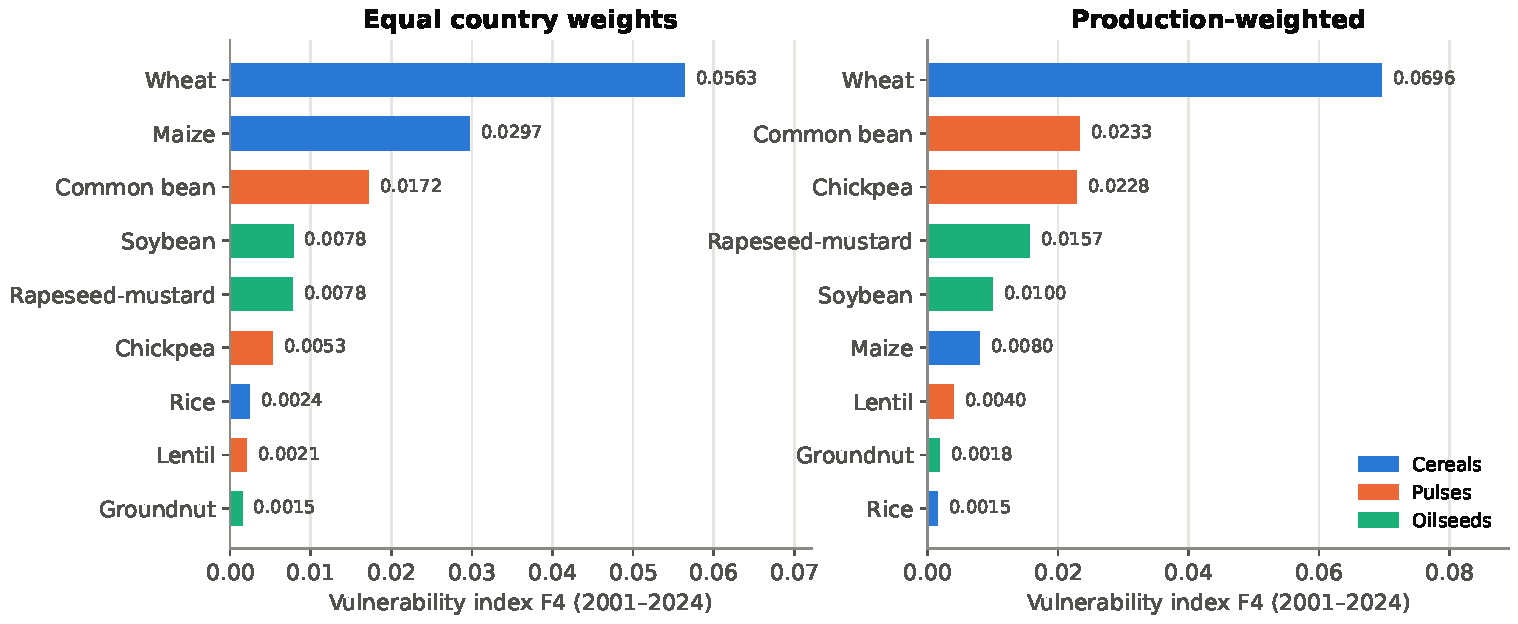
\includegraphics[width=\linewidth]{G01_crop_ranking.pdf}
\caption{Nine-crop vulnerability, 2001--2024 (\Fd). Left: mean over each crop's countries; right: weighted by
each country's production. Colour = crop group.}\label{fig:ranking}
\end{figure}

\paragraph{Order.} With equal country weights the order is \orderEq. Weighted by production it is \orderPw\
(Figure~\ref{fig:ranking}, Table~\ref{tab:cropindex}).

\paragraph{Stability.} Wheat is first under both weightings, in \robTopFfour\ of \robNFfour\ one-at-a-time
robustness rankings of \Fd, and in \mcTopShare\% of 2,000 random weightings (Section~\ref{sec:checks}). Positions
below first are much less stable:
\begin{itemize}
\item \secondEq\ is second with equal weights, but \secondPw\ is second with production weights;
\item rice is near the bottom under both weightings, for reasons explained below.
\end{itemize}

\begin{table}[H]\centering\small
\caption{Crop scores and components, 2001--2024 (equal weights unless marked pw).}\label{tab:cropindex}
\adjustbox{max width=\linewidth}{\begin{tabular}{llrrrrrrrrrr}
\toprule
Crop & Group & n & $E_T$ & $E_P$ & $S_T$ & $S_P$ & $\tilde I$ & F4 eq & rank & F4 pw & rank \\
\midrule
Wheat & Cereals & 6 & 0.03 & 0.23 & 0.50 & 0.88 & 0.53 & 0.0563 & 1 & 0.0696 & 1 \\
Maize & Cereals & 6 & 0.00 & 0.27 & 0.38 & 1.00 & 0.15 & 0.0297 & 2 & 0.0080 & 6 \\
Common bean & Pulses & 7 & 0.39 & 0.29 & 0.56 & 0.92 & 0.07 & 0.0172 & 3 & 0.0233 & 2 \\
Soybean & Oilseeds & 7 & 0.00 & 0.24 & 1.00 & 0.68 & 0.11 & 0.0078 & 4 & 0.0100 & 5 \\
Rapeseed-mustard & Oilseeds & 7 & 0.02 & 0.48 & 0.50 & 0.72 & 0.05 & 0.0078 & 5 & 0.0157 & 4 \\
Chickpea & Pulses & 7 & 0.00 & 0.52 & 0.70 & 0.70 & 0.02 & 0.0053 & 6 & 0.0228 & 3 \\
Rice & Cereals & 7 & 0.00 & 0.05 & 0.35 & 1.00 & 0.28 & 0.0024 & 7 & 0.0015 & 9 \\
Lentil & Pulses & 7 & 0.00 & 0.58 & 0.85 & 0.80 & 0.01 & 0.0021 & 8 & 0.0040 & 7 \\
Groundnut & Oilseeds & 5 & 0.01 & 0.16 & 0.47 & 0.56 & 0.09 & 0.0015 & 9 & 0.0018 & 8 \\
\bottomrule
\end{tabular}
\par\vspace{2pt}{\footnotesize Component columns are equal-weighted means over the crop's panel countries. eq = equal country weights; pw = production-weighted (FAOSTAT 2020--24).}
}
\end{table}

\subsection{What drives the scores}
\begin{figure}[H]\centering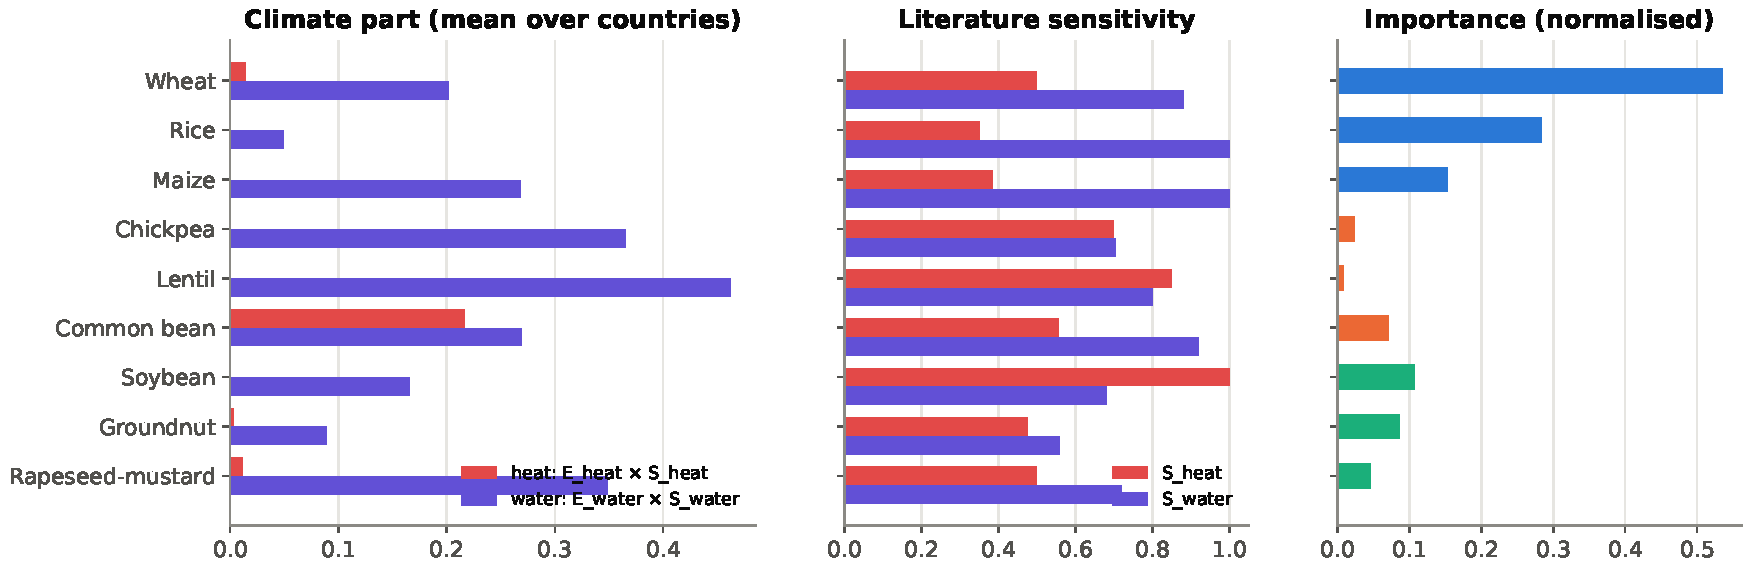
\includegraphics[width=\linewidth]{G03_components.pdf}
\caption{Climate part, sensitivity and importance by crop (equal-weighted means of the pair values).}\label{fig:components}\end{figure}

Figure~\ref{fig:components} separates the three components.
\begin{itemize}
\item \textbf{Wheat} combines high importance with exposure on both hazards. In the 2021--23 food balance sheets it
is the largest single food source of zinc in \wheatTopZinc, of iron in \wheatTopIron\ and of protein in
\wheatTopProtein\ of the \nDivUnits\ units (panel countries and World).
\item \textbf{Maize} is second with equal weights, mainly through two countries.
  \begin{itemize}
  \item South Africa: maize supplies \maizeSAkcal\% of national energy, \maizeSArainfed\% of its area is rainfed,
  and $E_{\text{water}}=\maizeSAEwater$.
  \item Ukraine: the largest water exposure of any maize pair (\maizeUAEwater).
  \end{itemize}
  With production weights maize drops, because in the two largest producers most maize is not eaten: only
  \maizeFoodUSA\% (USA) and \maizeFoodChina\% (China) of domestic supply goes to food.
\item \textbf{Soybean} has the steepest heat slope but zero heat exposure. Its monthly flowering $\Teff$ stays below
\SI{35}{\celsius} in all its countries, and it is eaten mainly as oil.
\item \textbf{Rice} scores low for two reasons, both properties of the measurement rather than proof that rice is
safe:
  \begin{itemize}
  \item most rice is irrigated, which the water measure counts as unstressed;
  \item monthly mean temperatures rarely exceed its \SI{35}{\celsius} anthesis threshold.
  \end{itemize}
\item \textbf{Pulses} enter the top half through common bean (heat) and chickpea (water). Their national importance
is small except in East Africa and South Asia, which keeps lentil low.
\end{itemize}

\subsection{Countries}
\begin{figure}[H]\centering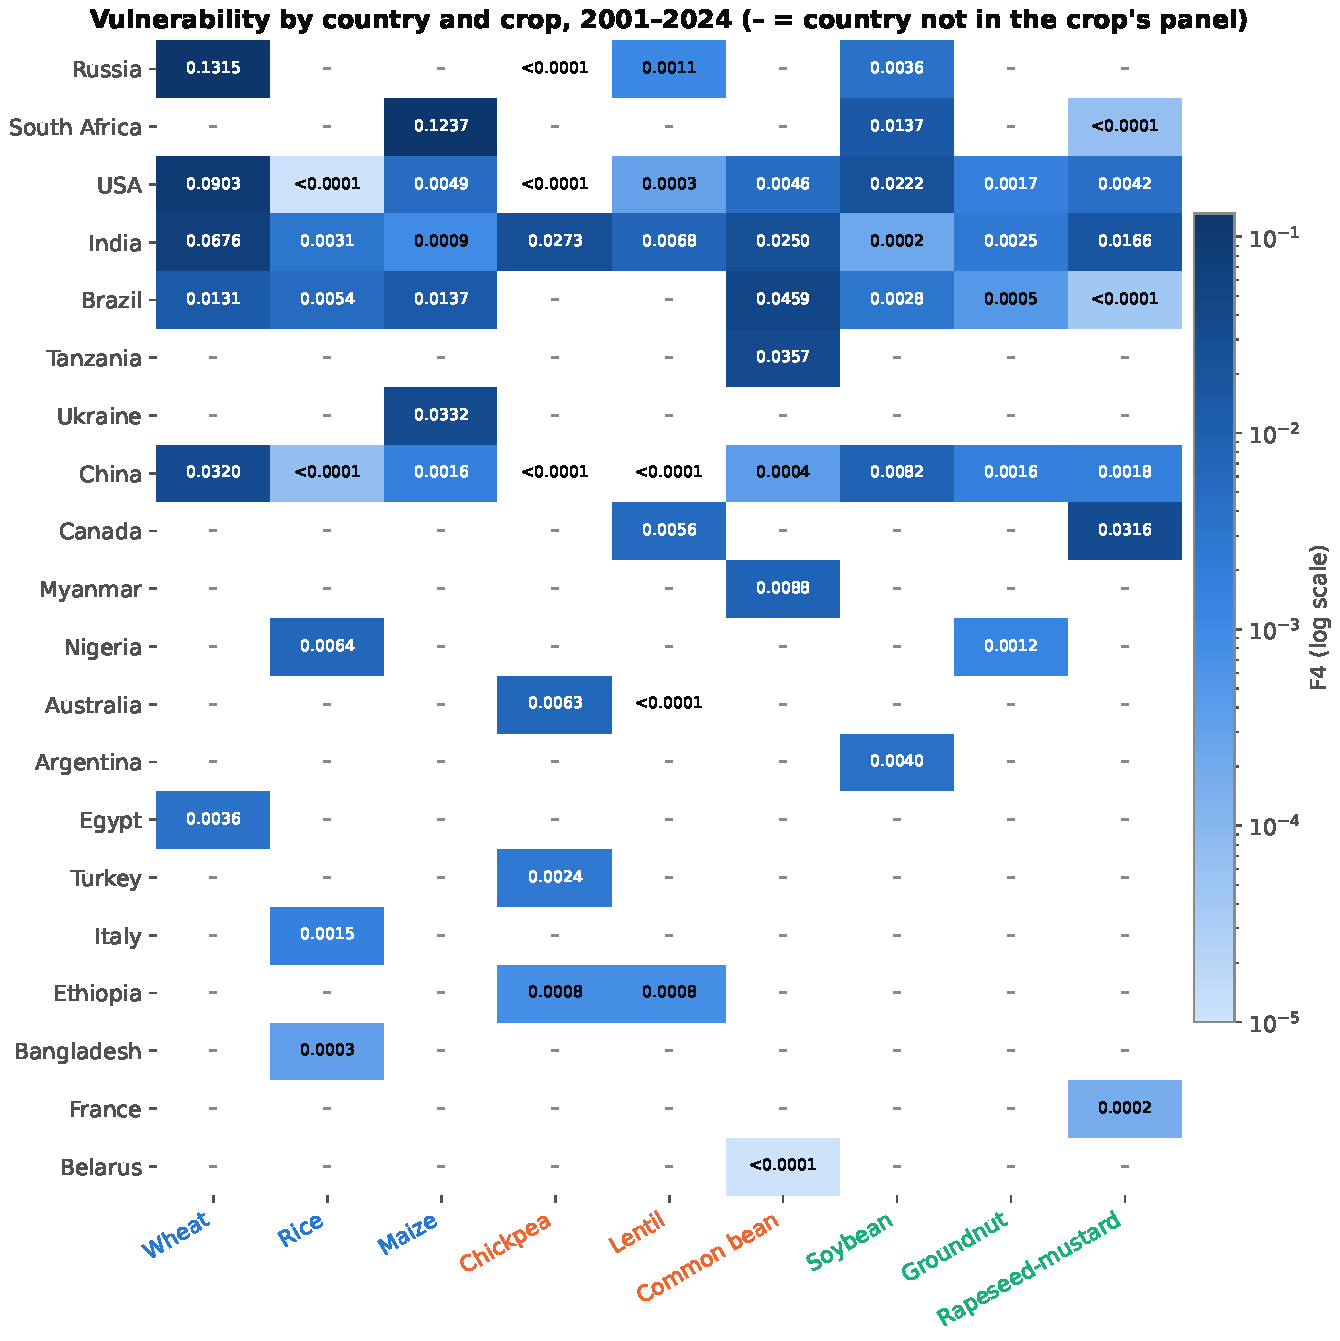
\includegraphics[width=0.92\linewidth]{G02_country_crop_matrix.pdf}
\caption{Country by crop \Fd, 2001--2024 (blank = crop not in that country's panel).}\label{fig:matrix}\end{figure}

\paragraph{Highest pairs.} The highest pairs are \topPairA\ (\topPairAValue), \topPairB\ (\topPairBValue), \topPairC\
(\topPairCValue), \topPairD\ (\topPairDValue), \topPairE\ (\topPairEValue) and \topPairF\ (\topPairFValue)
(Figure~\ref{fig:matrix}). They share one pattern: a crop that is a large part of the national diet \emph{and}
grown on rainfed land where its water need is often unmet. Examples are wheat in the Russian, US and Indian plains,
maize in South Africa, and beans in Brazil and Tanzania.

\paragraph{Water versus heat.} In \nTopSevenWater\ of the seven highest pairs the water term is larger than the heat
term. Over all pairs, water accounts for \presentWaterShare\% of the summed score today. Wheat in India has the
highest wheat heat exposure, but even there the water term is larger once heat is scaled by the panel's highest
heat level. The full country-by-crop table is Table~\ref{tab:countrycrop} (Appendix~\ref{app:tables}).

\subsection{Crop groups}
\begin{figure}[H]\centering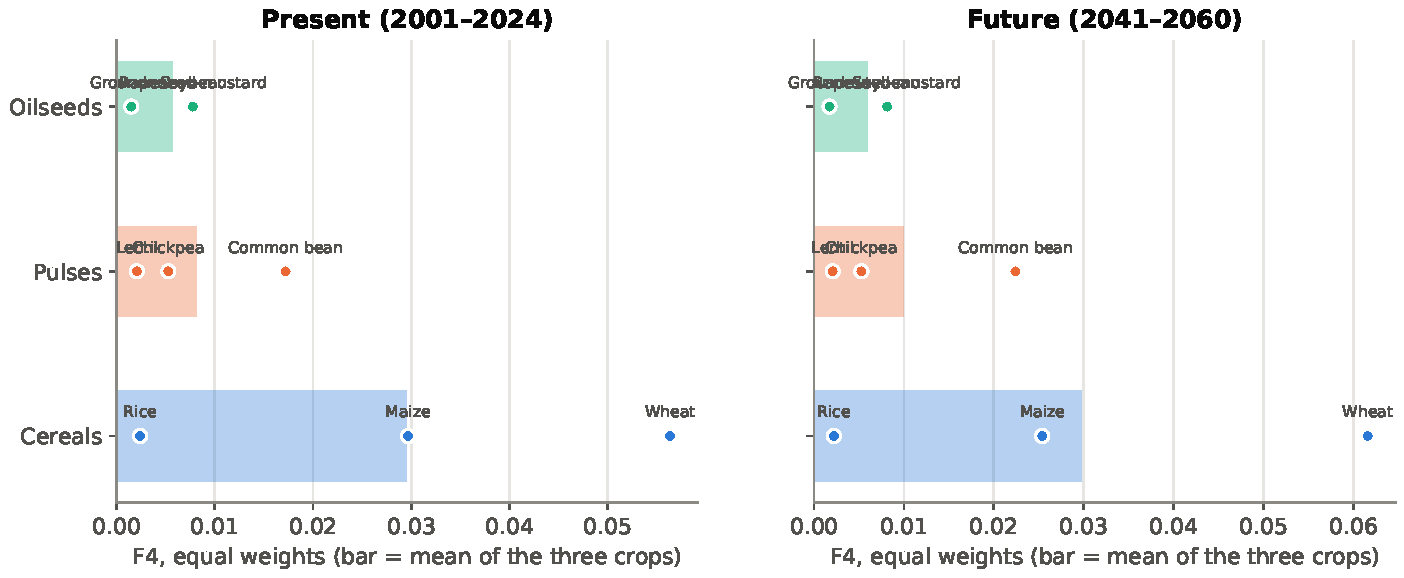
\includegraphics[width=0.85\linewidth]{G06_crop_groups.pdf}
\caption{Crop-group scores (mean of the three selected crops; bars show the range of the crops).}\label{fig:groups}\end{figure}

By group the order is \groupOrder\ (Figure~\ref{fig:groups}, Table~\ref{tab:groups}).
\begin{itemize}
\item The cereal lead comes from wheat and maize.
\item The pulse score comes from common bean and chickpea.
\item The oilseed score is low because soybean and rapeseed are eaten mainly as oil and have little heat
exposure.
\end{itemize}
A group mean describes three selected crops, so it should not be read as a statement about all cereals, pulses
or oilseeds.

\begin{table}[H]\centering\small\caption{Crop-group summaries (equal and production-weighted, with the range over
the three crops).}\label{tab:groups}
\adjustbox{max width=\linewidth}{\begin{minipage}{\textwidth}\centering
\adjustbox{max width=\textwidth}{\begin{tabular}{llrrrrr}
\toprule
Group & Crops & mean F4 eq & crop range & mean F4 pw & 1971--2000 & 2041--2060 \\
\midrule
Cereals & Wheat, Rice, Maize & 0.0295 & 0.0024--0.0563 & 0.0264 & 0.0275 & 0.0297 \\
Pulses & Chickpea, Lentil, Common bean & 0.0082 & 0.0021--0.0172 & 0.0167 & 0.0080 & 0.0099 \\
Oilseeds & Soybean, Groundnut, Rapeseed-mustard & 0.0057 & 0.0015--0.0078 & 0.0092 & 0.0059 & 0.0060 \\
\bottomrule
\end{tabular}
}
\par\vspace{2pt}{\footnotesize Group value = simple mean of the three selected crops; it describes these crops, not every cereal, pulse or oilseed.}
\end{minipage}
}\end{table}

\subsection{How adding crops changed the numbers}
The physical stress of every original pair is unchanged between the four-crop and nine-crop runs, but the
normalisation reference is not.
\begin{itemize}
\item The largest heat level is now \refHeatPair\ (\refHeat\,\si{\celsius} above its threshold), and the largest
water level \refWaterPair\ (\refWater).
\item All original scores therefore roughly halve, while their order is unchanged: \orderOrigFourEq\ in the
four-crop run, \orderOrigNineEq\ within the nine-crop run.
\end{itemize}

The bean reference is itself uncertain. It comes from a chamber-derived threshold for a heat-susceptible Andean
bean, applied to FAO ``beans, dry'', which in India includes tropical \emph{Vigna} pulses. Raising bean's threshold
by \SI{2}{\celsius}, or all new legumes' by \SI{3}{\celsius}, leaves wheat first (Table~\ref{tab:robust}).

Compared with the frozen mid-evaluation numbers, the presented literature-only method gives the same four-crop order
(\orderFourEq), with values higher by a median factor of \litRatioMedian\ (Figure~\ref{fig:midlit},
Appendix~\ref{app:tables}).
